%%=============================================================================
%% Resultaten
%%=============================================================================

\chapter{Resultaten}%
\label{ch:resultaten}

\section{\IfLanguageName{dutch}{Selectie van pentesting-tool}{Selection of pentesting-tool}}
Na het analyseren van de benodigdheden en het opstellen van een plan van aanpak kunnen de resultaten worden aangekaart. Er is 
hiervoor reeds besloten welke pentesting-tools met elkaar vergeleken worden. Zo is er gekozen voor Burp Suite, Metasploit en 
OWASP ZAP op basis van vooraf opgestelde criteria. Deze pentesting-tools worden eerst vergeleken aan de hand van richtlijnen 
die voor elke gebruiker belangrijk zijn bij het kiezen van een pentesting-tool.

Nadat deze resultaten zijn onderzocht in verband met de keuze van de de pentesttool, zal er worden overgegaan naar een tweede 
fase, waarbij de resultaten worden vergeleken met bevindingen van derden. Deze uitgebreidere resultaten zullen worden gebruikt 
om een pentesting-tool te identificeren die het beste past binnen het kader van deze proef.

\subsection{\IfLanguageName{dutch}{Resultaat volgens eigen criteria}{Result with own criteria}}
De drie geselecteerde pentesting-tools worden met elkaar vergeleken op het gebied van capaciteiten en functionaliteiten die 
ze aanbieden. Hierbij worden de tools grondig geëvalueerd, en worden de functionaliteiten van elk afzonderlijk getest. Het 
resourcegebruik wordt vergeleken op basis van CPU- en geheugengebruik. Ten slotte wordt ook de ondersteuning door de 
community beoordeeld, waarbij de gemiddelde responstijd op gemelde issues als maatstaf dient.

\subsubsection{\IfLanguageName{dutch}{Scala aan capaciteiten en functionaliteiten}{Scala aan capaciteiten en functionaliteiten}}
Burp Suite biedt het grootste aantal pentesting mogelijkheden wanneer men beschikt over de Professional Edition. Deze 
versie bevat geavanceerde functies zoals actieve scanning en geautomatiseerde aanvallen, die niet beschikbaar zijn in de 
gratis Community Edition. De Community Edition biedt echter wel essentiële tools zoals spidering waarmee alle endpoints 
en functies binnen een dynamische webapplicatiegedetecteerd kunnen worden, maar zonder ondersteuning 
voor AJAX (Asynchronous JavaScript and XML) spidering. Met AJAX spidering heb je de mogelijkheid om de content van de pagina 
te laten zonder de pagina volledig te vernieuwen. De proxyfunctionaliteit van Burp Suite stelt gebruikers in staat om webverkeer te onderscheppen en te 
analyseren. Dit is vooral handig bij het identificeren van kwetsbaarheden in dynamische webapplicaties. Gebruikers kunnen bij de 
host die ze willen spideren selecteren via de Target-tab en met een eenvoudige rechtermuisklik kiezen voor "Spider this host."

OWASP ZAP (Zed Attack Proxy) biedt daarentegen het breedste scala aan functionaliteiten in zijn gratis versie, waardoor het 
een aantrekkelijke keuze is voor organisaties die niet beschikken over een budget voor een commerciële tool. ZAP ondersteunt zowel 
passieve als actieve scanning, waarbij passieve scanners kwetsbaarheden detecteren door alleen het verkeer te analyseren en 
actieve scanners proberen potentiële kwetsbaarheden te exploiteren door actief verkeer te genereren. Bovendien biedt ZAP AJAX 
spidering, waarmee inhoud kan worden geladen zonder dat de hele pagina hoeft te worden vernieuwd, wat cruciaal is voor 
moderne en dynamische webapplicaties.

Metasploit richt zich voornamelijk op netwerkexploitatie en biedt uitgebreide mogelijkheden voor het uitvoeren van netwerkgerichte 
aanvallen en exploits. Hoewel het minder functies biedt op het gebied van webapplicatietests, zoals spidering en scanning, 
heeft Metasploit modules zoals http\_directory, http\_link\_scanner en http\_version die nuttig kunnen zijn voor het verzamelen 
van informatie over webservers en specifieke directories. Het ontbreken van een ingebouwde proxy en geavanceerde 
webscanningfunctionaliteiten maakt Metasploit echter minder geschikt voor gedetailleerde webapplicatietests in vergelijking 
met Burp Suite en OWASP ZAP.

Wanneer we de functionaliteiten van deze tools vergelijken, blijkt dat OWASP ZAP over het algemeen het meest bruikbaar is voor 
webapplicatietests, tenzij men toegang heeft tot de Burp Suite Professional Edition.
\subsubsection{\IfLanguageName{dutch}{Resourcegebruik}{Resourcegebruik}}
\begin{figure}
    \centering
    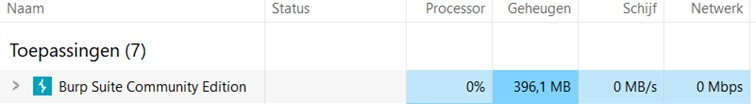
\includegraphics[height=0.1\textheight]{Burp_suite_rust.jpg}
    \caption[Resource gebruik van Burp suite in rust]{Resource gebruik van Burp suite in rust}
    \label{fig:burp_suite_rust}
\end{figure}
\begin{figure}
    \centering
    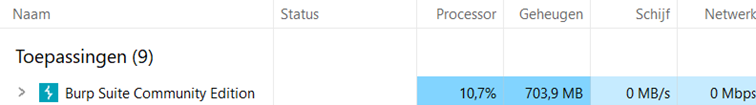
\includegraphics[height=0.1\textheight]{burp_suite_in_actie.png}
    \caption[Resource gebruik van Burp suite tijdens het uitvoeren van een actie]{Resource gebruik van Burp suite tijdens het uitvoeren van een actie}
    \label{fig:burp_suite_actie}
\end{figure}
\begin{figure}
    \centering
    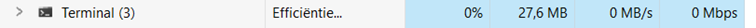
\includegraphics[height=0.025\textheight]{Metasploit_rust.png}
    \caption[Resource gebruik van Metasploit in rust]{Resource gebruik van Metasploit in rust}
    \label{fig:metasploit_rust}
\end{figure}
\begin{figure}
    \centering
    
\includegraphics[height=0.02\textheight]{Metasploit_in_actie.png}
    \caption[Resource gebruik van Metasploit tijdens het uitvoeren van een actie]{Resource gebruik van Metasploit tijdens het uitvoeren van een actie}
    \label{fig:metasploit_actie}
\end{figure}
\begin{figure}
    \centering
    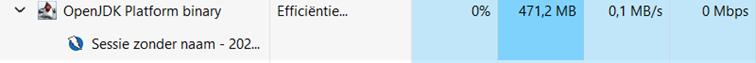
\includegraphics[height=0.05\textheight]{OWASP_ZAP_rust.png}
    \caption[Resource gebruik van OWASP ZAP in rust]{Resource gebruik van OWASP ZAP in rust}
    \label{fig:owasp_rust}
\end{figure}
\begin{figure}
    \centering
    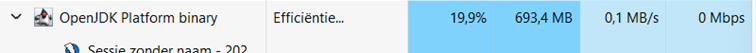
\includegraphics[height=0.05\textheight]{OWASP_ZAP_in_actie.png}
    \caption[Resource gebruik van OWASP ZAP tijdens het uitvoeren van een actie]{Resource gebruik van OWASP ZAP tijdens het uitvoeren van een actie}
    \label{fig:owasp_actie}
\end{figure}
Om het resourcegebruik van de drie pentesting-tools te vergelijken, wordt zowel het verbruik in rust als het verbruik tijdens het 
uitvoeren van een actie gemeten. De eerste tool waarvan het resourcegebruik is gemeten is Burp Suite. Hierbij zijn zowel de 
prestaties in rust als tijdens actieve taken geregistreerd. De resultaten van deze metingen zijn te zien in de afbeeldingen. 
Dit is in rust \ref{fig:burp_suite_rust} en dit is tijdens het uitvoeren van een actie \ref{fig:burp_suite_actie}. 

Voor het vergelijken van het resourcegebruik is ook Metasploit onderworpen aan metingen in zowel rust als tijdens actieve 
penetratietests. Metasploit wordt uitgevoerd in de terminal, daarom zijn de resource resultaten te zien onder de terminal tab 
in taakbeheer. Deze metingen geven inzicht in de efficiëntie van Metasploit onder verschillende omstandigheden. De 
resultaten van het resourcegebruik in rust zijn te vinden in figuur \ref{fig:metasploit_rust}, terwijl het verbruik tijdens 
actieve testen wordt weergegeven in figuur \ref{fig:metasploit_actie}.

OWASP ZAP is eveneens geanalyseerd op zijn resourcegebruik, zowel in rust als tijdens het uitvoeren van beveiligingstests. 
Deze metingen helpen bij het bepalen van de belasting die ZAP op het systeem legt onder verschillende operationele scenario's. 
De resultaten van het resourcegebruik van OWASP ZAP in rust zijn weergegeven in figuur \ref{fig:owasp_rust}, en tijdens het 
uitvoeren van acties in figuur \ref{fig:owasp_actie}.

\subsubsection{\IfLanguageName{dutch}{Ondersteuning van de community }{Ondersteuning van de community}}
\begin{figure}
    \centering
    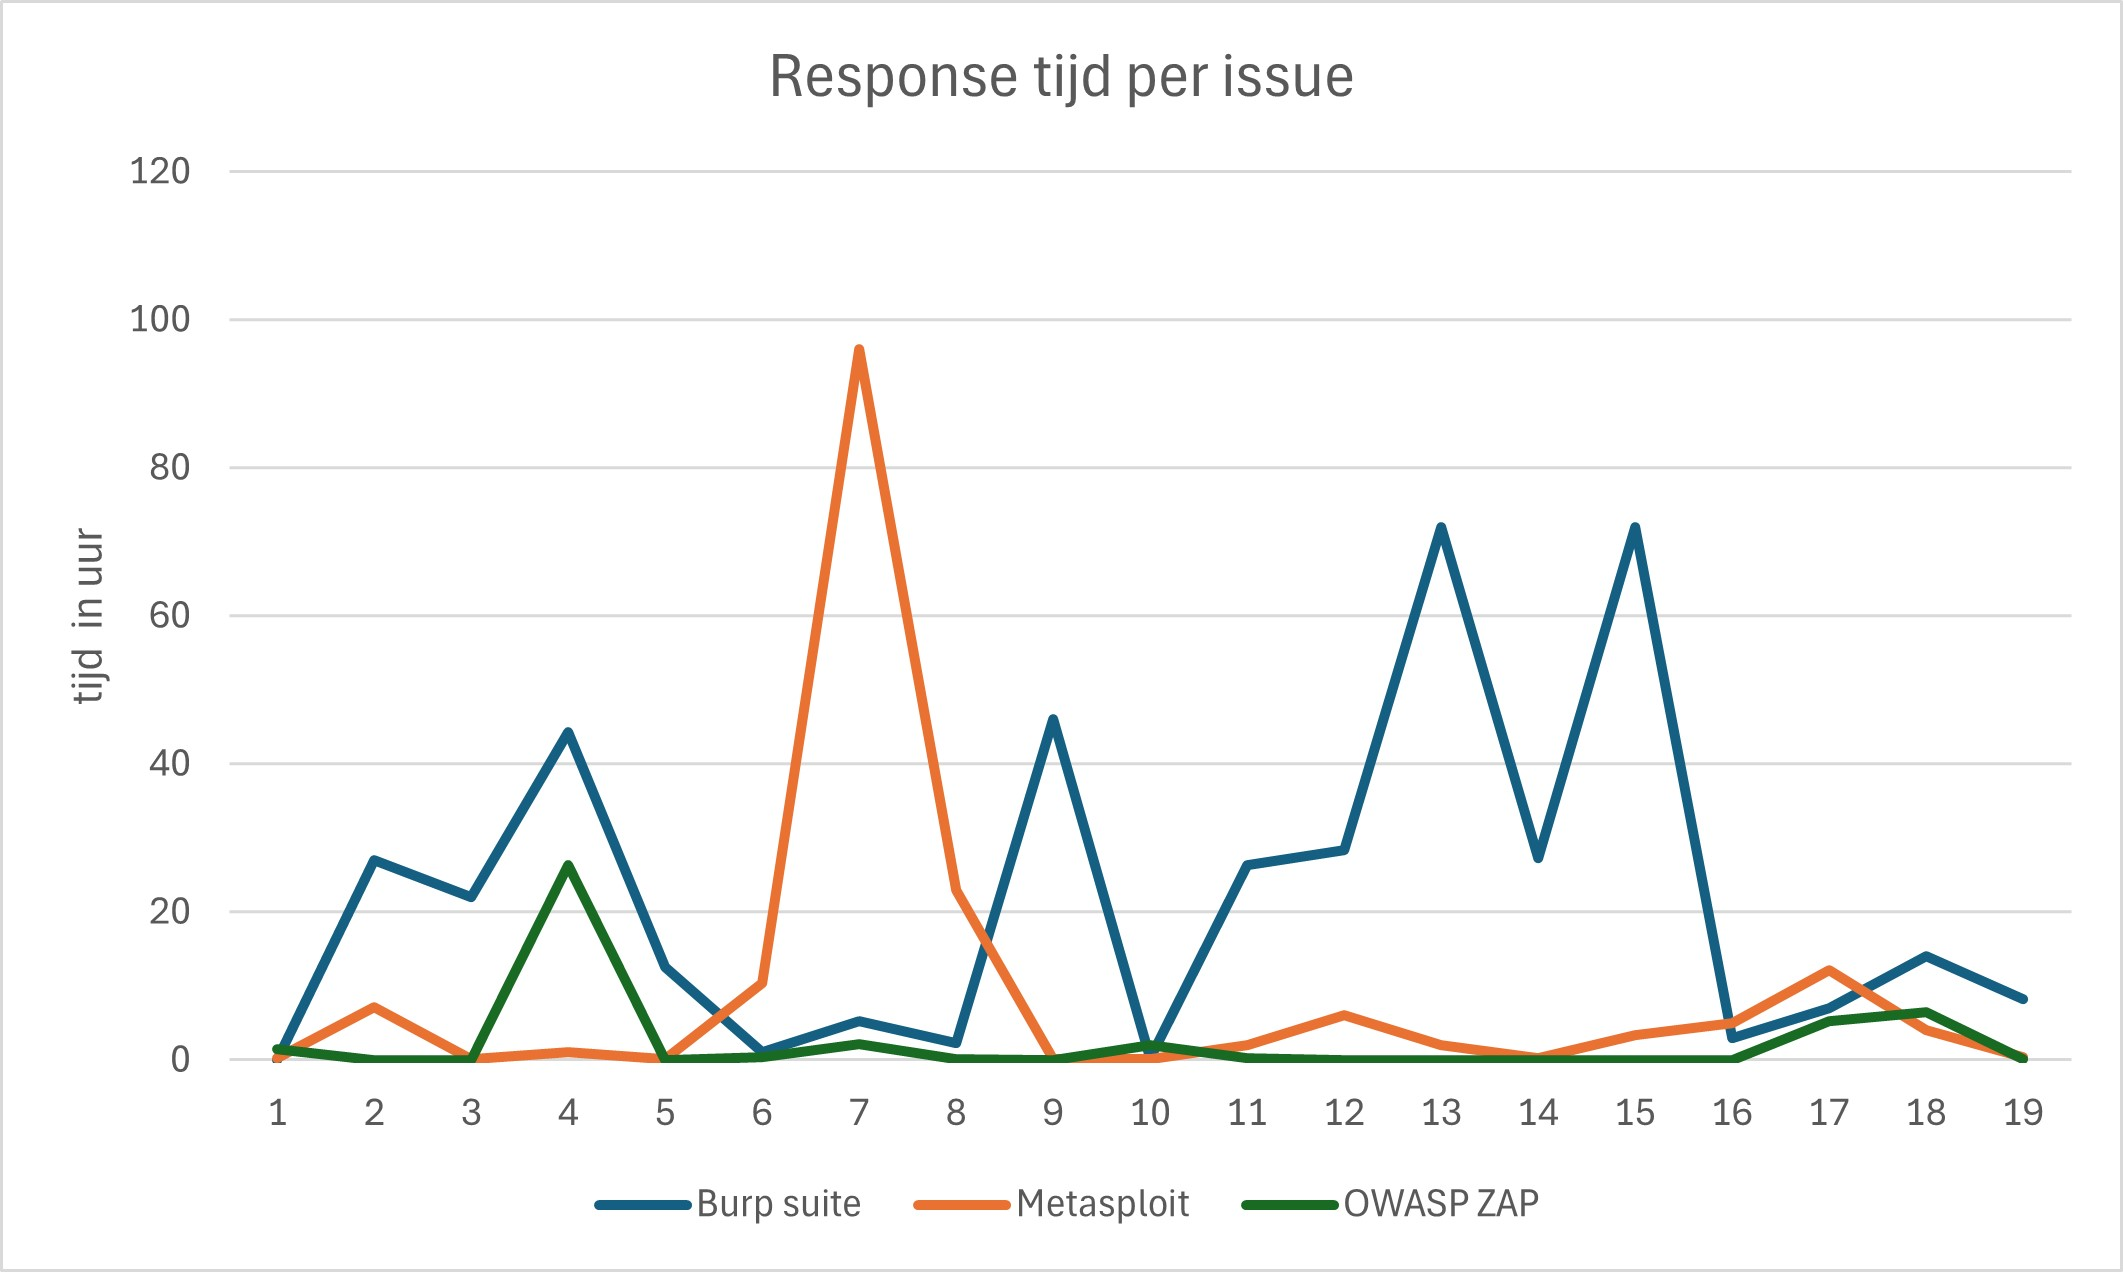
\includegraphics[height=0.3\textheight]{grafiek_respons_resultaten.jpg}
    \caption[Grafiek van 19 willekeurige issues bij de pentesttools en de tijd hoe lang het duurt om te repliceren]{Grafiek van 19 willekeurige issues bij de pentesttools en de tijd hoe lang het duurt om te repliceren}
    \label{fig:respons_grafiek}
\end{figure}
De ondersteuning van de developers of de community is een belangrijke factor bij het kiezen van een pentesting-tool. Om de ondersteuning 
te evalueren, zijn 19 willekeurige issues gemeld bij de drie pentesting-tools. De tijd die nodig is om deze
vragen te beantwoorden, is vastgelegd en geanalyseerd. De resultaten van deze analyse zijn te zien in de
grafiek \ref{fig:respons_grafiek}. Hieruit blijkt dat OWASP ZAP de snelste responstijd heeft, gevolgd door Metasploit en
Burp Suite. Dit zijn de gemiddelde response tijden van de 19 issues die zijn gemeld bij de drie pentesting-tools.
\begin{itemize}
    \item OWASP ZAP: 2u 46 min
    \item Metasploit: 8u
    \item Burp Suite: 22u 15 min
\end{itemize}

Aangezien OWASP ZAP en Metasploit open-source tools zijn, zijn de issues te vinden op github en is de community actief
betrokken bij het oplossen van problemen. Burp Suite is een commerciële tool en heeft een eigen support team dat 
verantwoordelijk is voor het oplossen van problemen. In tegenstelling tot Metasploit en OWASP ZAP worden de issues niet 
op github gepost, maar op een apart platform portswigger. Dit kan de responstijd beïnvloeden, 
aangezien de issues eerst opgepakt moeten worden door het support team.

\subsubsection{\IfLanguageName{dutch}{Globale resultaten}{Global results}}
Na het analyseren van de capaciteiten en functionaliteiten, het resourcegebruik en de ondersteuning van de community,
kunnen de resultaten van de drie pentesting-tools worden samengevat. De vergelijking van de drie tools toont aan dat
OWASP ZAP de meest uitgebreide functionaliteiten biedt voor het testen van webapplicaties, gevolgd door Burp Suite 
community edition en Metasploit. 

De resultaten van de resource metingen tonen aan dat Metasploit het minste 
geheugen en CPU verbruikt in vergelijking met Burp Suite en OWASP ZAP. Het verbruik van OWASP ZAP ligt iets hoger dan 
Burp Suite, maar is nog steeds acceptabel voor de meeste systemen. 

De responstijd van de community is het snelst bij OWASP ZAP, 
gevolgd door Metasploit en Burp Suite. Dit toont aan dat OWASP ZAP de meest actieve community heeft die snel reageert op 
gemelde problemen.

Deze resultaten bieden een overzicht van de prestaties van de drie pentesting-tools en helpen bij het bepalen van de 
meest geschikte tool voor het uitvoeren van beveiligingstests op webapplicaties. Op basis van deze resultaten kan een 
definitieve conclusie worden getrokken over welke tool het meest geschikt is voor de tests. Volgens de eigen criteria 
lijkt OWASP ZAP de beste keuze te zijn voor het uitvoeren van beveiligingstests op webapplicaties, gevolgd door Burp Suite 
community edition en Metasploit. 

\subsection{\IfLanguageName{dutch}{Resultaat volgens derden}{Result with third parties}}
Na de vergelijking van de drie pentesting-tools volgens de eigen criteria, worden de resultaten getoetst aan bevindingen van 
derden.

De resultaten van externe gebruikers worden bepaald door drie factoren te analyseren: voordelen, nadelen en een algemene 
beoordeling van elke tool. Deze factoren trachten inzicht te bieden in de ervaringen van andere gebruikers met de drie pentesting-tools. 
De bevindingen van derden worden gebruikt om de betrouwbaarheid van de eigen resultaten al dan niet te bevestigen en een definitieve conclusie 
te trekken om één tool te weerhouden voor de tests.

De resultaten van derden zijn gebaseerd op informatie van G2.com en Peerspot. Er is gekozen voor meerdere bronnen om een zo 
breed mogelijk beeld te krijgen van de gebruikerservaringen met de drie pentesting-tools. De resultaten van derden worden 
samengevat in de volgende secties. Eerst worden de uitkomsten van G2.com besproken, gevolgd door de resultaten van Peerspot. 
Daarna worden deze resultaten samengevoegd en vergeleken met de eigen bevindingen om een definitieve pentesting-tool te 
selecteren.

\subsubsection{\IfLanguageName{dutch}{G2}{G2}}
De voordelen van Burp Suite betreffen het gebruiksgemak en de gebruiksvriendelijke interface. De nadelen zijn echter 
de hoge kosten van de Professional Edition, de beperkte functionaliteiten in de Community Edition en de trage prestaties. De 
algemene beoordeling van Burp Suite community edition komt uit op 4,8/5.

OWASP ZAP wordt gewaardeerd om zijn gebruiksvriendelijkheid, uitgebreide automatiseringsmogelijkheden en efficiëntie. 
Dit maakt het een aantrekkelijke keuze voor organisaties die op zoek zijn naar een tool die geschikt is voor beginnende en 
ervaren gebruikers. Aan de andere kant zijn de nadelen de beperkte documentatie en de gelimiteerde scope van de tool. De 
algemene beoordeling van OWASP ZAP is 4,7/5.

Metasploit staat bekend om zijn efficiëntie en kwalitatieve resultaten. Echter, de tool wordt ook als complex ervaren en 
heeft een steile leercurve, wat een uitdaging kan zijn voor minder ervaren gebruikers. De algemene beoordeling van Metasploit 
is 4,6/5.

\subsubsection{\IfLanguageName{dutch}{Peerspot}{Peerspot}}
De resultaten van Peerspot tonen aan dat Burp Suite wordt gewaardeerd om zijn gebruiksvriendelijkheid en extensies die zeer 
nuttig zijn voor het uitvoeren van beveiligingstests. De tool wordt echter ook als duur ervaren en heeft het vermogen om foutieve 
positieven te genereren bij het scannen van grote applicaties. Met foutieve positieve wordt bedoeld dat de uitslag van een 
test/experiment die ten onrechte positief is. De algemene beoordeling van Burp Suite is 4,3/5.

OWASP ZAP wordt geprezen om zijn uitgebreide functionaliteiten en gebruiksgemak. Het biedt de mogelijkheid om kwetsbaarheden 
te detecteren die andere tools mogelijk missen en beschikt over een breed scala aan automatiseringsopties, zoals automatische, 
actieve en passieve scans. Daarnaast is OWASP ZAP compatibel met Linux, Windows en Mac. De nadelen zijn echter de beperkte 
documentatie, de steile leercurve voor beginnende gebruikers en de kans op foutieve positieve. De algemene beoordeling van 
OWASP ZAP is 3,8/5.

Metasploit wordt gewaardeerd om zijn automatiseringsmogelijkheden en het vermogen om kwetsbaarheden te scannen zonder 
bijkomende setup. De technische ondersteuning van Metasploit is ook uitstekend volgens de beoordelingen op peerspot. De tool 
is echter minder geschikt voor beginners, aangezien het minder gebruiksvriendelijk is. Daarnaast bevat Metasploit een 
aanzienlijk aantal verouderde exploits. De algemene beoordeling van Metasploit is 3,8/5.

\subsection{\IfLanguageName{dutch}{Definitieve pentesttool}{}}
\label{sec:Definitieve_pentesttool}
Na het analyseren van de resultaten van derden en de opgestelde criteria, blijkt dat OWASP ZAP de best passende tool is voor het uitvoeren van 
beveiligingstests op webapplicaties binnen de context van een KMO webdeveloper zoals Sinergio. De tool biedt een uitgebreide reeks functionaliteiten en is gebruiksvriendelijk, wat 
het een aantrekkelijke keuze maakt voor organisaties die op zoek zijn naar een kosteneffectieve oplossing voor het uitvoeren 
van beveiligingstests. Ook de automatiseringsmogelijkheden en efficiëntie van OWASP ZAP dragen bij aan de positieve 
beoordeling van de tool.

\section{\IfLanguageName{dutch}{Resultaten van webomgevingen}{Results of web environments}}
\subsection{\IfLanguageName{dutch}{Algemene waarschuwingen na scan}{Algemene waarschuwingen na scan}}

\begin{figure}
    \centering
    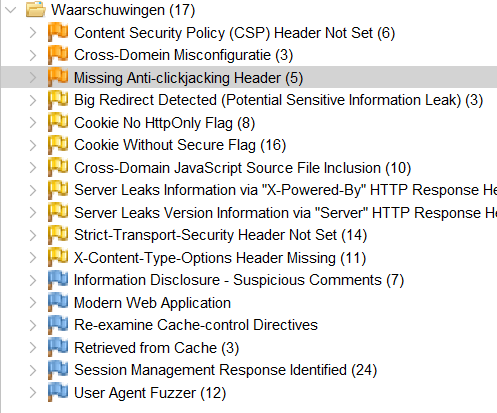
\includegraphics[height=0.3\textheight]{waarschuwingen_laravel.png}
    \caption[Alle waarschuwingen die gedetecteert zijn na een actieve scan en ajax spider in owasp zap bij de laravel applicatie]
    {Alle waarschuwingen die gedetecteert zijn na een actieve scan en ajax spider in owasp zap bij de laravel applicatie}
    \label{fig:waarschuwingen_laravel}
\end{figure}
\begin{figure}
    \centering
    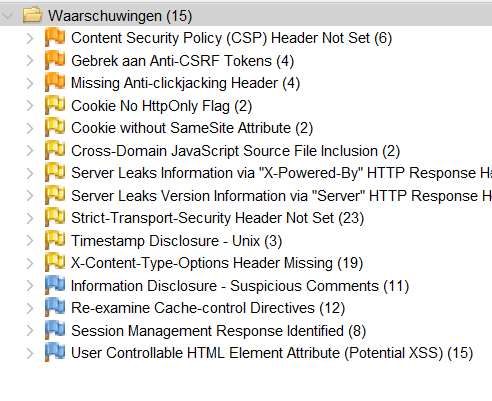
\includegraphics[height=0.3\textheight]{waarschuwingen_zonder_plugin.png}
    \caption[Alle waarschuwingen die gedetecteert zijn na een actieve scan en ajax spider in owasp zap bij de wordpress applicatie zonder beveiligingsplugins]
    {Alle waarschuwingen die gedetecteert zijn na een actieve scan en ajax spider in owasp zap bij de wordpress applicatie zonder beveiligingsplugins}
    \label{fig:waarschuwingen_zonder}
\end{figure}
\begin{figure}
    \centering
    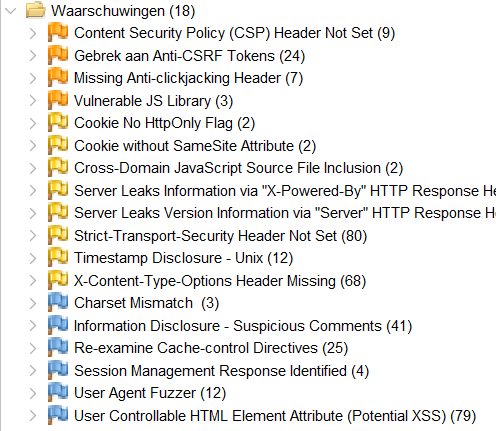
\includegraphics[height=0.3\textheight]{waarschuwingen_met_plugin.png}
    \caption[Alle waarschuwingen die gedetecteert zijn na een actieve scan en ajax spider in owasp zap bij de wordpress applicatie met beveiligingsplugins]
    {Alle waarschuwingen die gedetecteert zijn na een actieve scan en ajax spider in owasp zap bij de wordpress applicatie met beveiligingsplugins}
    \label{fig:waarschuwingen_met}
\end{figure}

Voor de resultaten van de webomgevingen onderzocht werden, werden de waarschuwingen die gedetecteerd zijn na een actieve scan en AJAX spider in OWASP ZAP 
geanalyseerd. De waarschuwingen geven inzicht in de kwetsbaarheden van de webapplicaties en helpen bij het identificeren van 
mogelijke beveiligingsrisico's. De resultaten van de waarschuwingen zijn te zien op de afbeeldingen. Zo is te zien dat er bij de 
laravel applicatie 17 waarschuwingen zijn gedetecteerd \ref{fig:waarschuwingen_laravel}. Bij de wordpress applicatie zonder 
beveiligingsplugins zijn er 15 waarschuwingen gedetecteerd \ref{fig:waarschuwingen_zonder}. Bij de wordpress 
applicatie met beveiligingsplugins zijn er 18 waarschuwingen gedetecteerd \ref{fig:waarschuwingen_met}.

Deze uitkomst geeft een beeld van alle mogelijke kwestbaarheden binnen de webapplicaties, maar geeft geen inzicht in de 
ernst van de kwetsbaarheden. Om de ernst van de kwetsbaarheden te bepalen, werden de waarschuwingen verder geanalyseerd. 
Deze waarschuwingen verschillen van applicatie tot applicatie aan de hand van de gebruikte technologieën en de 
beveiligingsmaatregelen die zijn genomen.

\subsection{\IfLanguageName{dutch}{SQL injectie}{SQL injection}}
\begin{figure}
    \centering
    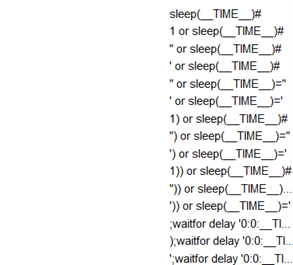
\includegraphics[height=0.2\textheight]{sql_injectie_laravel.png}
    \caption[SQL injectie aanval op laravel applicatie]{SQL injectie aanval op laravel applicatie}
    \label{fig:injectie_laravel}
\end{figure}
\begin{figure}
    \centering
    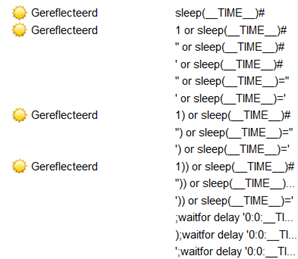
\includegraphics[height=0.2\textheight]{sql_injectie_met_plugin.png}
    \caption[SQL injectie aanval op wordpress applicatie met beveiligingsplugins]{SQL injectie aanval op wordpress applicatie met beveiligingsplugins}
    \label{fig:injectie_zonder}
\end{figure}
\begin{figure}
    \centering
    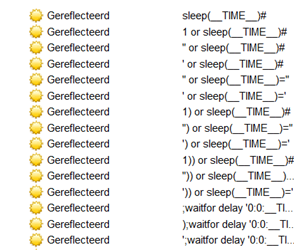
\includegraphics[height=0.2\textheight]{sql_injectie_zonder_plugin.png}
    \caption[SQL injectie aanval op wordpress applicatie zonder beveiligingsplugins]{SQL injectie aanval op wordpress applicatie zonder beveiligingsplugins}
    \label{fig:injectie_met}
\end{figure}


Een van de meest voorkomende kwetsbaarheden in webapplicaties, op basis van de OWASP top 10, is SQL-injectie. Om de 
kwetsbaarheid van de webapplicaties 
te testen, werd een SQL-injectie aanval uitgevoerd op de laravel applicatie \ref{fig:injectie_laravel} en de 
wordpress applicatie met en zonder beveiligingsplugins \ref{fig:injectie_zonder}, \ref{fig:injectie_met}. 

Wanneer een SQL-script als kwetsbaar wordt beschouwd, zal dit worden weergegeven in het outputvenster met gereflecteerd ernaast. 
Dit betekent niet dat de SQL-injectie succesvol is uitgevoerd, maar dat er een mogelijkheid bestaat om een SQL-injectie te laten 
slagen. 

De resultaten van de SQL-injectie aanval tonen aan dat de laravel applicatie het minst kwetsbaar is voor SQL-injectie, terwijl 
de wordpress applicatie zonder beveiligingsplugins het meest kwetsbaar is. De wordpress applicatie met beveiligingsplugins 
biedt een gemiddelde bescherming tegen SQL-injectie aanvallen, wat aantoont dat de beveiligingsplugins effectief zijn in het 
voorkomen van de meeste scripts. 

\subsection{\IfLanguageName{dutch}{Security misconfiguratie}{Security misconfiguration}}
\begin{figure}
    \centering
    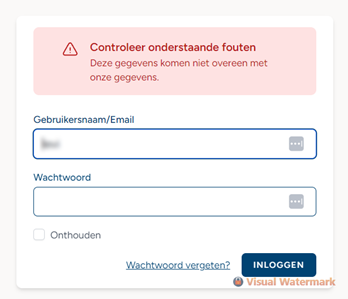
\includegraphics[height=0.2\textheight]{fout_pass_laravel.png}
    \caption[foutief password met correcte gebruikersnaam melding bij laravel]{foutief password met correcte gebruikersnaam melding bij laravel}
    \label{fig:sec_mis_laravel}
\end{figure}
\begin{figure}
    \centering
    
\includegraphics[height=0.2\textheight]{fout_pass_met.png}
    \caption[foutief password met correcte gebruikersnaam melding met wordfence]{foutief password met correcte gebruikersnaam melding met wordfence}
    \label{fig:sec_mis_met}
\end{figure}
\begin{figure}
    \centering
    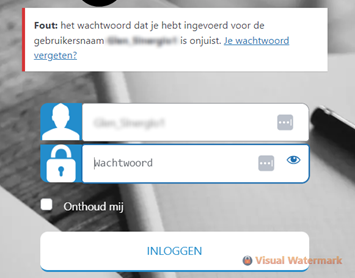
\includegraphics[height=0.2\textheight]{fout_pass_zonder.png}
    \caption[foutief password met correcte gebruikersnaam melding zonder wordefence]{foutief password met correcte gebruikersnaam melding zonder wordfence}
    \label{fig:sec_mis_zonder}
\end{figure}
\begin{figure}
    \centering
    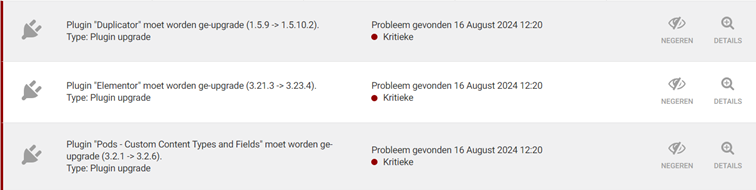
\includegraphics[height=0.1\textheight]{verouderde_plugins.png}
    \caption[Meldingen dat wordfence geeft wanneer er verouderde plugins gebruikt worden]{Meldingen dat wordfence geeft wanneer er verouderde plugins gebruikt worden}
    \label{fig:verouderde_plugins}
\end{figure}
\begin{figure}
    \centering
    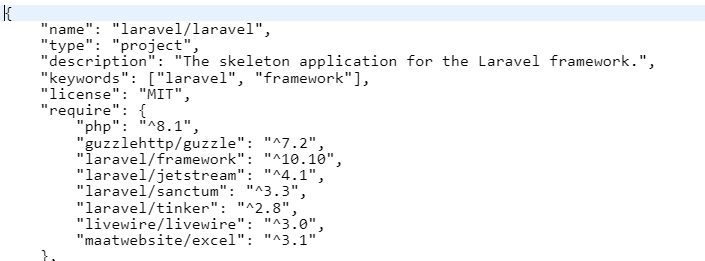
\includegraphics[height=0.2\textheight]{versie_laravel.png}
    \caption[Versie gebruik van de laravel applicatie]{Versie gebruik van de laravel applicatie}
    \label{fig:versie_laravel}
\end{figure}
Een andere veelvoorkomende kwetsbaarheid in webapplicaties is security misconfiguratie. Om deze vulnerabilitie te vergelijken 
bij de webapplicaties werdt er gekeken naar welke melding weergegeven word na het ingeven van een foutief wachtwoord
en correcte gebruikersnaam. De resultaten hiervan zijn te zien in de afbeeldingen. Zo is te zien dat bij de laravel 
applicatie een foutmelding wordt getoond die door de developer zelf is ingested \ref{fig:sec_mis_laravel}. Bij de wordpress 
applicatie zonder beveiligingsplugins wordt er een foutmelding getoond die aangeeft dat het wachtwoord fout is in combinatie 
met de opgegeven gebruikersnaam \ref{fig:sec_mis_zonder}. Bij de wordpress applicatie met beveiligingsplugins wordt er een 
foutmelding getoond die aangeeft dat de gebruikersnaam of wachtwoord fout is \ref{fig:sec_mis_met}.

Een andere vorm van security misconfiguratie is het gebruik van verouderde plugins. Dit kan leiden tot kwetsbaarheden in 
de webapplicatie. Om dit te testen werd er gekeken naar de versie van de plugins die gebruikt worden in de wordpress 
applicatie. De resultaten hiervan zijn te zien in de afbeelding \ref{fig:verouderde_plugins}. Hieruit blijkt dat de wordfence 
plugin aangeeft welke plugins verouderde versie hebben in tegenstelling tot de wordpress applicatie zonder beveiligingsplugins. 
Bij de wordpress applicatie zonder beveiligingsplugins is het niet duidelijk welke plugins verouderd zijn en kan dit leiden 
tot kwetsbaarheden in de webapplicatie.

Hetzelde geldt voor de laravel applicatie, voor de eigenaar van de website is het gewoonlijk niet duidelijk welke versie van 
het laravel framework gebruikt wordt. De versie van laravel wordt gebruikelijk geüpdate door de developer, maar het is 
belangrijk om te weten welke versie van laravel gebruikt wordt om kwetsbaarheden te voorkomen. Op bovenstaande afbeelding is 
te zien dat de versie van laravel verouderd is en dat er een update beschikbaar is \ref{fig:versie_laravel}. Dit kan leiden 
tot kwetsbaarheden in de webapplicatie. 


\subsection{\IfLanguageName{dutch}{sensitive data exposure}{sensitive data exposure}}
Sensitive data exposure is een kwetsbaarheid waarbij gevoelige informatie, zoals wachtwoorden en persoonlijke gegevens, wordt 
blootgesteld aan ongeautoriseerde gebruikers. Om deze kwetsbaarheid te testen werd onderzocht hoe wachtwoorden worden 
opgeslagen in de database van de webapplicaties. Ook werd gekeken naar de manier waarop de informatie via het netwerk wordt 
verzonden. Dit werd onderzocht door de serverconfiguratie te beoordelen. Hierbij zijn specifieke regels ingesteld om ervoor 
te zorgen dat websites op accountniveau niet via HTTP toegankelijk zijn en dat er geen niet-versleutelde gegevens tussen de 
server en de applicatie worden verzonden.

De wachtwoorden in dit geval zijn opgeslagen aan de hand van een hash en een salt in de database. Dit betekent dat de 
wachtwoorden niet in plain text worden opgeslagen en dat de wachtwoorden niet zichtbaar zijn voor ongeautoriseerde gebruikers. 
De gegevens worden ook versleuteld verzonden via HTTPS, wat betekent dat de gegevens veilig zijn tijdens het transport tussen 
server en applicatie. Voorbeelden van hoe de wachtwoorden worden opgeslagen en verzonden zijn te zien in de afbeelding 
......., ook de rules die ingesteld zijn op de server zijn te zien op deze foto ...... .


\subsection{\IfLanguageName{dutch}{Cross site scripting (XSS)}{Cross site scripting (XSS)}}
\begin{figure}
    \centering
    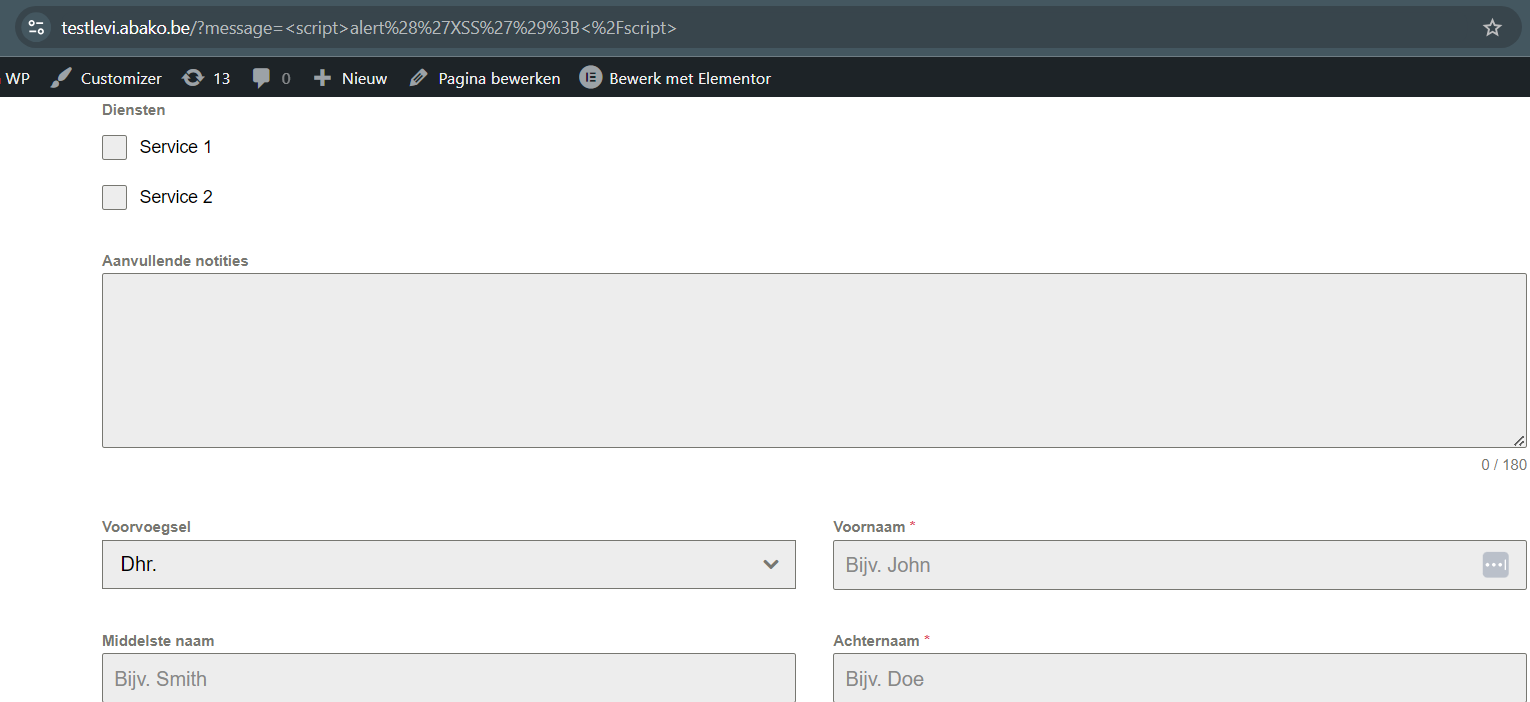
\includegraphics[height=0.2\textheight]{mislukte_XSS.png}
    \caption[Een mislukte reflected XSS test]{Een mislukte reflected XSS test}
    \label{fig:mislukte_XSS}
\end{figure}
\begin{figure}
    \centering
    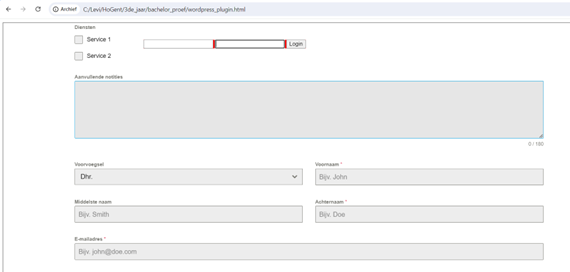
\includegraphics[height=0.2\textheight]{I_frame_met.png}
    \caption[Een voorbeeld van een opgezette I-frame]{Een voorbeeld van een opgezette I-frame}
    \label{fig:i_frame_met}
\end{figure}
\begin{figure}
    \centering
    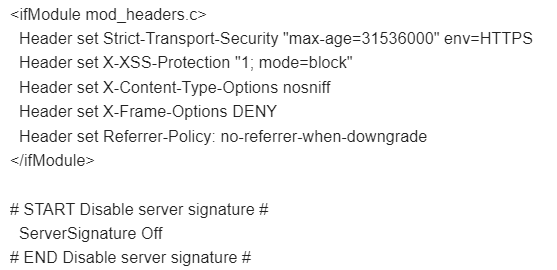
\includegraphics[height=0.2\textheight]{headers_htaccess.png}
    \caption[.htaccess lijnen die te maken hebben met het mogelijkmaken om een I-frame te nemen]{.htaccess lijnen die te maken hebben met het mogelijkmaken om een I-frame te nemen}
    \label{fig:headers_htaccess}
\end{figure}

Cross-Site Scripting (XSS) is een kwetsbaarheid waarbij kwaadwillende scripts worden geïnjecteerd in webpagina's die door 
gebruikers worden bezocht. Om deze kwetsbaarheid te testen, is een XSS-aanval uitgevoerd op de webapplicaties. De resultaten 
van de aanval werden geverifieerd door te controleren of er een alert-box op de webpagina verscheen. De uitkomst van de 
XSS-aanval is weergegeven in afbeelding \ref{fig:mislukte_XSS}. Hieruit blijkt dat de XSS-aanval is mislukt en dat de webapplicaties
bescherming bieden tegen XSS-aanvallen.

Een ander voorbeeld van een XSS-aanval betreft het uit zetten van de X-Frame-Options op de server. Deze optie bepaalt of 
elementen van jouw website mogen worden ingeladen via een frame. Als deze optie niet is ingesteld, kan de webapplicatie in 
een iframe op een andere website worden ingeladen, wat kan leiden tot clickjacking en andere vormen van aanvallen. Om dit te 
testen, is gekeken naar de ingestelde headers op de server. De resultaten hiervan zijn te zien in afbeelding \ref{fig:i_frame_met}. 
Hieruit blijkt dat de X-Frame-Options niet zijn ingesteld op de server, waardoor de webapplicatie kan worden ingeladen in een 
iframe op een andere website. Dit kan ertoe leiden dat, wanneer een gebruiker zijn gebruikersnaam en wachtwoord
invoert, deze informatie wordt gelogd op de server van de aanvaller.

Om dit risico te beperken, zijn er headers ingesteld op de server om te voorkomen dat de webapplicatie in een iframe op een 
andere website kan worden ingeladen. De ingestelde headers zijn weergegeven in afbeelding \ref{fig:headers_htaccess}. De 
headers kunnen aangepast worden in de .htaccess file op de server, dit is een configuratie bestand gebruikt door apache 
gebaseerde web servers.

\subsection{\IfLanguageName{dutch}{Onvoldoende logging en monitoring}{Insufficient logging and monitoring}}
\begin{figure}
    \centering
    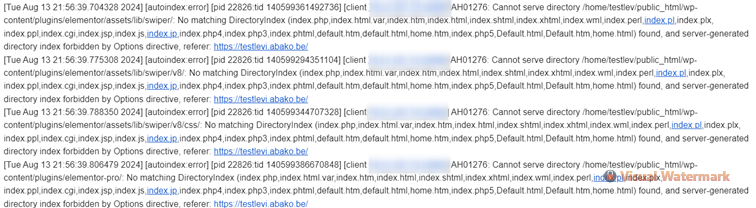
\includegraphics[height=0.2\textheight]{server_logging.png}
    \caption[de error log van de server tijdens het uitvoern van een actieve scan]{de error log van de server tijdens het uitvoern van een actieve scan}
    \label{fig:server_logging}
\end{figure}
Insufficient logging and monitoring is een kwetsbaarheid waarbij onvoldoende logging en monitoring worden toegepast op de 
webapplicatie. Om deze kwetsbaarheid te testen, is de error log van de server gecontroleerd tijdens het uitvoeren van een 
actieve scan op de webapplicaties. De resultaten van de error log zijn te zien in afbeelding \ref{fig:server_logging}. 
Hieruit blijkt dat de serverlogging actief is en dat er geen tekortkomingen waren tijdens de uitvoering van de actieve scan. 
Dit betekent dat de webapplicatie over voldoende logging en monitoring beschikt om verdachte activiteiten te detecteren en te 
rapporteren.

In de error log van de server werd bijvoorbeeld weergegeven dat er op dat moment een AJAX-spider elke mogelijke pagina aan 
het bezoeken was. In de logs is ook zichtbaar vanaf welk IP-adres de verzoeken afkomstig zijn en welke pagina's de spider 
probeert te vinden op de betreffende website. Deze informatie wordt gelogd in de error log van de server en kan worden 
gebruikt om verdachte activiteiten te detecteren.

\subsection{\IfLanguageName{dutch}{Brute force}{Brute force}}
\begin{figure}
    \centering
    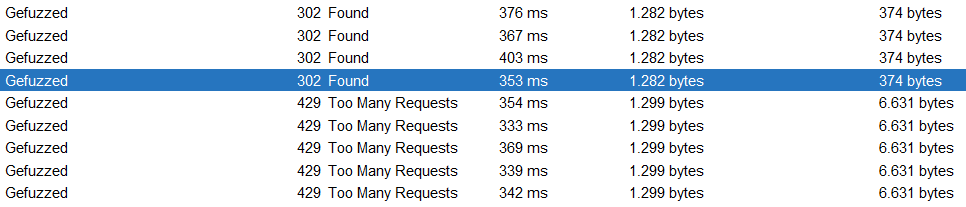
\includegraphics[height=0.2\textheight]{brute_force_laravel.png}
    \caption[Brute force aanval op laravel applicatie]{Brute force aanval op laravel applicatie}
    \label{fig:brute_force_laravel}
\end{figure}
\begin{figure}
    \centering
    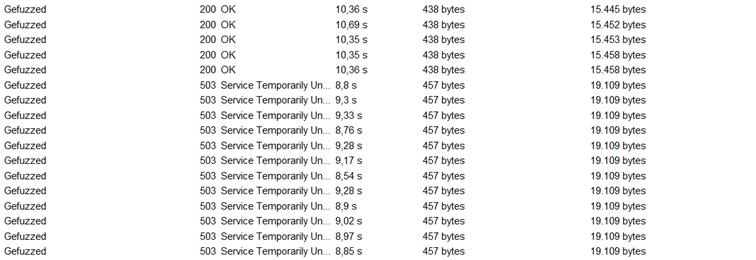
\includegraphics[height=0.2\textheight]{brute_force_met.png}
    \caption[Brute force aanval op wordpress applicatie met beveiligingsplugins]{Brute force aanval op wordpress applicatie met beveiligingsplugins}
    \label{fig:brute_force_met}
\end{figure}
\begin{figure}
    \centering
    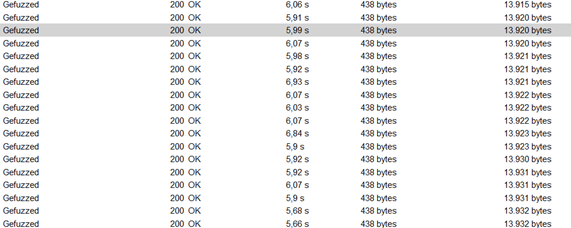
\includegraphics[height=0.2\textheight]{brute_force_zonder.png}
    \caption[Brute force aanval op wordpress applicatie zonder beveiligingsplugins]{Brute force aanval op wordpress applicatie zonder beveiligingsplugins}
    \label{fig:brute_force_zonder}
\end{figure}

Brute force is een kwetsbaarheid waarbij aanvallers proberen toegang te krijgen tot een systeem door herhaaldelijk gebruikersnamen 
of wachtwoorden te raden. Om deze kwetsbaarheid te testen, is een brute force-aanval uitgevoerd op de webapplicaties met OWASP ZAP. De 
resultaten van deze aanval zijn weergegeven in afbeelding\ref{fig:brute_force_met} en \ref{fig:brute_force_zonder}. 

Uit de resultaten blijkt duidelijk dat de WordPress-applicatie met beveiligingsplugins bescherming biedt tegen brute 
force-aanvallen door na vijf mislukte pogingen verdere inlogpogingen te blokkeren. Daarentegen is het bij de 
WordPress-applicatie zonder beveiligingsplugins mogelijk om onbeperkt inlogpogingen te doen zonder consequenties. Dit toont 
aan dat de beveiligingsplugins effectief zijn in het voorkomen van brute force-aanvallen.

Ook bij de Laravel-applicatie is het niet mogelijk om een brute force-aanval uit te voeren, aangezien de applicatie na vier 
mislukte pogingen de gebruiker eveneens zal blokkeren zoals te zien is op de foto \ref{fig:brute_force_laravel}.
